\documentclass[a4paper,14pt]{article}
\usepackage{extsizes}
\usepackage{amsmath}
\usepackage{amssymb}
\everymath{\displaystyle}
\usepackage{geometry}
\usepackage{fancyhdr}
\usepackage{multicol}
\usepackage{graphicx}
\usepackage[brazil]{babel}
\usepackage[shortlabels]{enumitem}
\usepackage{cancel}
\columnsep=2cm
\hoffset=0cm
\textwidth=8cm
\setlength{\columnseprule}{.1pt}
\setlength{\columnsep}{2cm}
\renewcommand{\headrulewidth}{0pt}
\geometry{top=1in, bottom=1in, left=0.7in, right=0.5in}

\pagestyle{fancy}
\fancyhf{}
\fancyfoot[C]{\thepage}

\begin{document}
	
	\noindent\textbf{7FMA152~-~Matemática} 
	
	\begin{center}Revisão: o plano $\mathbb{R}^2$ (Versão estudante)
	\end{center}
	
	
	\noindent\textbf{Nome:} \underline{\hspace{10cm}}
    \noindent\textbf{Data:} \underline{\hspace{4cm}}
	
	%\section*{Questões de Matemática}
	
	\begin{multicols}{2}
	    \begin{enumerate}
	    	\item Sendo $A = \{1, 5\}$, $B = \{2, 4\}$ e $C = \{4, 5\}$, apresentar:
	    	\begin{enumerate}[a)]
	    		\item $B \times C$ \\\\\\\\\\
	    		\item $A \times B$ \\\\\\\\\\
	    		\item $C \times A$ \\\\\\\\\\
	    		\item $B^2$ \\\\\\\\\\
	    		\item $\big(A \times B\big) \cap \big(B \times C\big)$ \\\\\\\\\\\\
	    	\end{enumerate}
    	    \item Apresentar no plano $\mathbb{R}^2$ os seguintes pontos:\\\\
    	    $A\big(1; 1\big)$\\
    	    $B\big(0; 0\big)$\\
    	    $C\big(-1; 0\big)$\\
    	    $D\big(-2; -4\big)$\\
    	    $E\big(2; -3\big)$\\
    	    $F\big(-3; 4\big)$\\
    	    $G\big(4; 2\big)$\\\\\\\\\\\\\\\\\\\\\\\\
    	    \item Se o ponto $\big(a; -b\big)$ está no segundo quadrante, onde estão os pontos $\big(a; b\big)$, $\big({-a}; b\big)$ e $\big({-a}; {-b}\big)$? \\\\\\\\\\\\\\\\
    	    \item Apresentar o simétrico $A'$ de $A = \big(2; 1\big)$ em relação ao eixo dos $x$, o simétrico $B'$ de $B = \big(5; 4\big)$ em relação ao eixo dos $y$ e o simétrico $C'$ de $C = \big({-2}; {-3}\big)$ em relação à origem. \\\\\\\\\\\\\\\\\\\\\\\\\\\\\\\\\\\\\\\\\\\\\\\\\\\\
    	    \item No gráfico estão representados os gols marcados e os gols sofridos por uma equipe de futebol nas dez primeiras partidas de um determinado campeonato.
    	    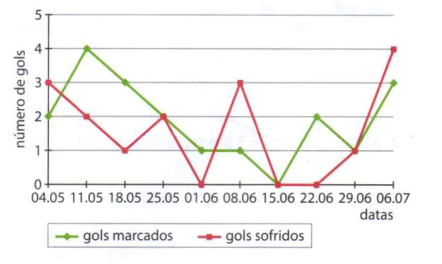
\includegraphics[width=0.45\textwidth]{/home/hogdelta/Documentos/latex/7FMA152_imagens/pg69-1.png}
    	    Considerando que, nesse campeonato, as equipes ganham 5 pontos para cada vitória, 2 pontos por empate e 0 ponto em caso de derrota, a equipe em questão, ao final da décima partida, terá acumulado um número de pontos igual a:\\
    	    \begin{enumerate}[a)]
    	    	\item 15
    	    	\item 18
    	    	\item 21
    	    	\item 26
    	    	\item 32
    	    \end{enumerate}
	        \item Sendo $A = \{2, 4, 6\}$ e $B = \{1, 2\}$, determine:
	        \begin{enumerate}[a)]
		    	\item $A \times B$ \\\\\\\\\\
		    	\item $B \times A$ \\\\\\\\\\
		    	\item $B^2$ \\\\\\\\\\
		    	\item $B^2 \cap A^2$ \\\\\\\\\\
	        \end{enumerate}
            \item Determine todas as relações de A = $\{1, 2, 3\}$ em B = $\{2, 3, 5\}$ tais que todo elemento de A forme par ordenado com exatamente um elemento de $B$ e vice-versa.
            \\\\\\\\\\\\\\\\\\\\
            \item Represente no plano $\mathbb{R}^2$ os pontos:\\
            $A = \big(2; 4\big)$\\
            $B = \big(0; 1\big)$\\
            $C = \big({-2}; 2\big)$\\
            $D = \big({-3}; 0\big)$\\
            $E = \big(1; {-5}\big)$\\
            $F = \big({-4}; {-2}\big)$\\
            $G = \big(0; {-3}\big)$\\
            $H = \big(1; 1\big)$\\
            $I = \big(0; 0\big)$\\
            $J = \big(4; {-4}\big)$\\\\\\\\\\\\\\\\\\\\\\
            \item Considere o ponto $P = (x; {-y})$
            \begin{enumerate}[a)]
            	\item Sabendo-se que o simétrico de $P$ em relação à origem está no 2º quadrante, o que podemos afirmar sobre $x$ e $y$?\\\\\\\\\\
            	\item Determine as coordenadas dos pontos simétricos de $P$ em relação à origem, ao eixo dos $x$ e ao eixo dos $y$.
            \end{enumerate}
        \end{enumerate} 
    $~$ \\ $~$ \\ $~$ \\ $~$ \\ $~$ \\ $~$ \\ $~$ \\ $~$ \\ $~$ \\ $~$ \\ $~$ \\ $~$ \\ $~$ \\
    \end{multicols}
\end{document}